
\subsection{Time Course Analyses}

\begin{figure}[ht]
  \centering
  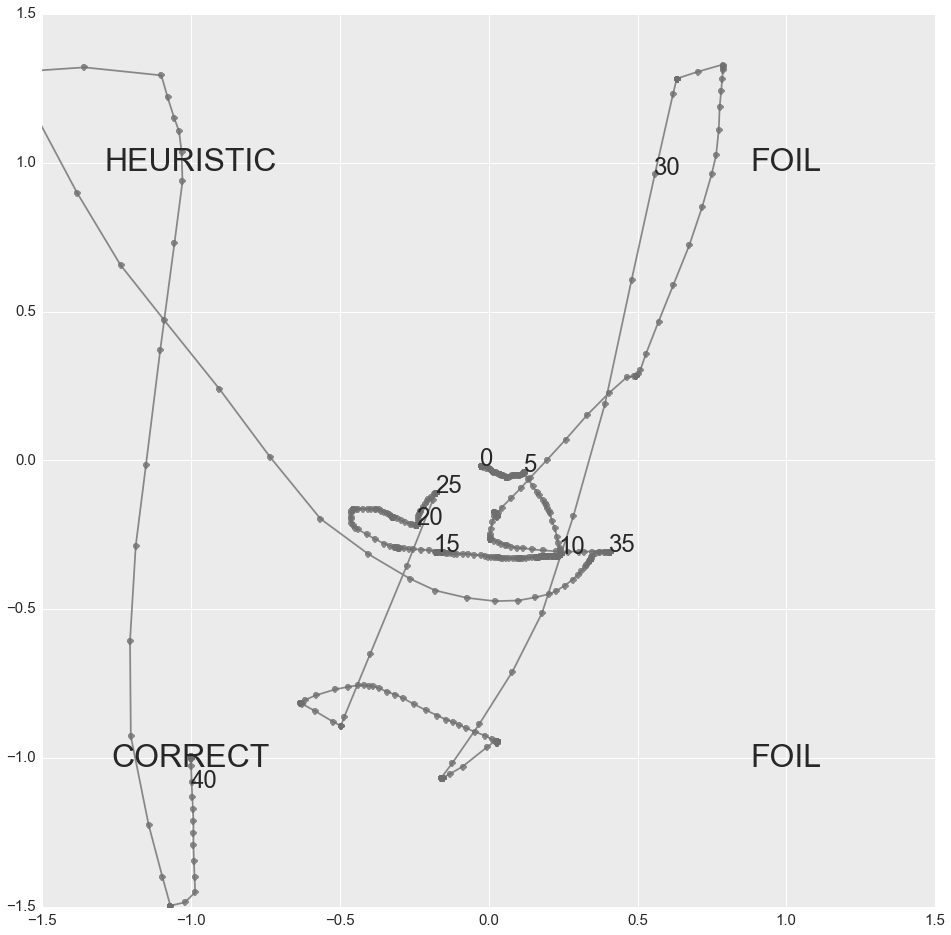
\includegraphics[width=\figurewidth]{imgs/exp6-typical-trajectory.png}
  \caption[A typical cursor trajectory from Experiment 6.]{
    \label{fig:exp6-typical-trajectory}
    A typical mouse cursor trajectory from the conflict condition. 
    Numerical values indicate the time elapsed in seconds. 
    Cursors meandered as participants generated their responses, 
    passing near the response options located in the corners of the display
  }
\end{figure}

In most previous mouse tracking research,
both in this thesis and in general
\citep[e.g.][]{Freeman2011d,Spivey2005},
the location of the cursor is recorded over a few seconds,
as participants move it from a starting position to 
a response option located in either top corner of the screen.
Almost invariably, this path follows either a single movement
(curved or otherwise) to a response,
or as has been more the case in this thesis,
a movement towards one response, that changes direction mid-flight.
In the current data, unfolding over up to 60 seconds, 
participants move and rest the cursor many times throughout a trial,
an average of 5.1 times, and a maximum of 30.
Thus, this data is in ways more similar to eye movement data.
A typical mouse cursor trajectory is shown in Figure~\ref{fig:exp6-typical-trajectory},
showing  a number of movements which pass near to several response options. 
In order to analyse participants' attraction to each response option over time,
the display was divided into quadrants
corresponding to each response option.
For the first 60 seconds of each trial, 
the mouse cursor positions at each 200 millisecond time slice
were coded according to which section of the screen they occupied, 
similar to fixation analyses of eye-tracking data.

Figure~\ref{fig:exp6-all} shows, for each response region, 
the proportion of trials in which the cursor is in that region, over time,
for both conflict and no-conflict problems. 
While the proportions at 60 seconds here 
largely reflect participants' ultimate responses, 
earlier proportions show how these preferences developed over time. 
Both correct responses to no-conflict problems and 
heuristic responses to conflict problems
were intuitively appealing, and participants 
began to move towards both options from before 5 seconds.
At approximately 10 seconds, participants also began to move towards
the correct response option on conflict problems,
and the accumulation of cursors in the region 
of the heuristic option under conflict slowed accordingly. 
The proportion of cursors in the region of these foil response options 
declined steadily in both conditions. 
Note that the proportions for the foil response options 
are averaged across the two foil options on conflict problems, 
and three options on no-conflict problems.

\begin{figure}[hp]
  \centering
  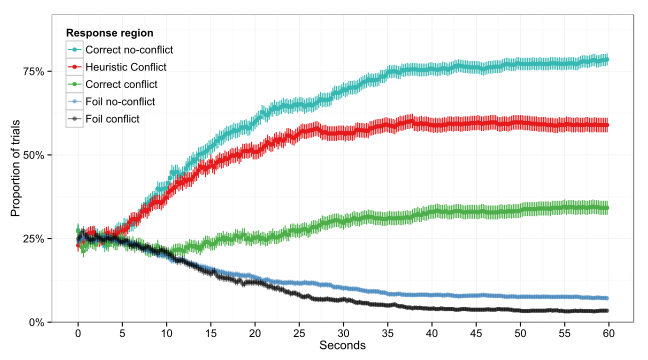
\includegraphics[width=\figurewidth]{imgs/exp6-all.pdf}
  \caption[Proportion of mouse cursors each region of the screen over time, Experiment 6.]{
    \label{fig:exp6-all}
    Proportion of mouse cursors in the region of the screen 
    corresponding to each response options, over time, 
    for conflict and no-conflict problems.    
  }
\end{figure}

\begin{figure}[bp]
  \centering
  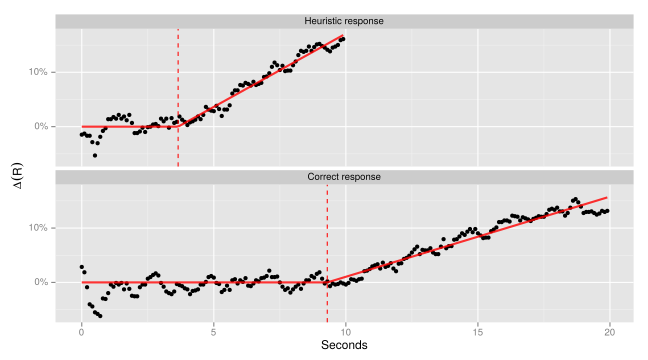
\includegraphics[width=\figurewidth]{imgs/exp6_changepoint.pdf}
  \caption[Change point analysis, Experiment 6.]{
    \label{fig:exp6_changepoint}
    Top: $\Delta (Heuristic)$, the difference between
    the probability of the cursor being in the region of the heuristic option
    and the probability of being in the region of a foil option.\\
    Bottom: $\Delta (Correct)$, the difference between
    the probability of being in the region of the correct option,
    and of being in the region of a foil option.
    Solid red lines show non-linear regression fits.
    Dashed vertical lines show change points,
    after which participants began to be drawn towards the option in question.
  }
\end{figure}

\subsubsection{Bayesian Change Point Analysis}

Inspecting Figure~\ref{fig:exp6-all},
participants are initially equally likely
to move toward each of the four response options
on conflict trials, doing so 25\% of the time.
This is the case until some time before 5 seconds,
at which point participants become more likely
to be in the region of the heuristic option
than the correct option, or either of the foils,
reflecting the point at which processes driving participants
towards the heuristic response exert their influence.
Similarly participants were equally likely to be
in the region of the correct option as the foils
until around 10 seconds,
and after this point more likely to be in the region of the correct option,
indicating that participants begin to be drawn towards the correct option
from this time.

Of course, visual inspection of these curves
is not a particularly accurate means of revealing
\emph{when} participants begin to be drawn towards each response option.
To formally estimate the times at which
participants began to move towards each response,
I calculated, across each 40 msec,
$\Delta (Heuristic)$: the difference between the average probability
of the cursor being in the region of the heuristic option
and the probability of being in the region of either foil option, as well as
$\Delta (Correct)$: the difference between the average probability
of being in the region of the correct option
and of being in the region of the foil option.
This yielded two series of values (Figure~\ref{fig:exp6_changepoint})
that were close to $0$ until participants
began to be drawn towards the response in question,
and increased over time after that point.

I modelled these series using a non-linear regression model
of the form

\begin{equation*}
  \Delta (R) =
  \begin{cases}%
    0          & \text{if}\ t\ <\ \tau_{R} \\
    \beta * (t-\tau_{R})  & \text{otherwise}%
  \end{cases}
\end{equation*}

where $t$ is the time in seconds,
$\tau_{R}$  is the point at which
participants begin to be drawn towards response $R$,
and $\beta$ is the slope of the regression line
after time $\tau_{R}$.

Modelling $\Delta (Heuristic)$, I analysed the first 10 seconds of each trial,
and set a uniform prior on the value of $\tau_{Heuristic}$ between 0 and 10 seconds
(i.e. that participants were equally likely to start being drawn
towards the heuristic response any time between 0 and 10 seconds into a trial).
Modelling $\Delta (Correct)$, I analysed the first 20 second,
and again set a uniform prior on $\tau_{Correct}$ between 0 and 20 seconds.
In both cases, I set an uninformative normal prior
with mean 0 and SD 1 on the slope, $\beta$.

Figure~\ref{fig:exp6_changepoint} shows the fitted regression models,
and Table~\ref{tbl:exp6_changepoint} shows the posterior estimates for the parameters.
The posteriors for the $\tau$ parameters represent
estimates of the point at which participants began to be drawn to each response.
The median posterior estimate for $\tau_{Heuristic}$ was
3.65 seconds (95\% credible interval [3.36, 3.93 seconds]),
and the estimate for $\tau_{Correct}$ was
9.30 seconds (95\% credible interval [8.86, 9.64 seconds]).
The $\beta$ parameters reflect how quickly
the proportion of participants in the region of each option increased after time $\tau$.
The estimate for $\beta_{Heuristic}$
(median 0.027, or a 2.7\% increase per second,
95\% credible interval [2.5\%, 2.9\%])
was almost twice as large as that for $\beta_{Correct}$
(median 0.015, or a 1.5\% increase per second,
95\% credible interval [1.4\%, 1.6\%]).
To summarise, participants began to be drawn towards
the heuristic option from 3.6 seconds,
and towards the correct option from 9.3 seconds.
After these onsets of attraction,
there was a greater increase in the proportion of trials
where the cursor was in the region of the heuristic option (2.7\% per second)
than in the proportion of trials
where it was in the region of the correct option (1.5\% per second).


\begin{table}
  \centering
  \caption[Bayesian change point analysis, Experiment 6.]{
    Posterior estimates from the change point analysis.
    Participants began to be drawn towards the heuristic option
    from 3.65 seconds, and the correct option from 9.30 seconds.
    \label{tbl:exp6_changepoint}
  }
  \begin{tabular}{lrrr}
    \toprule
    Parameter           & Median & 2.5\% & 97.5\%\\
    \midrule
    $\tau_{Heuristic}$  & 3.65  & 3.36 & 3.93\\
    $\tau_{Correct}$    & 9.30  & 8.86 & 9.64\\
    \midrule
    $\beta_{Heuristic}$ & 0.027  & 0.025 & 0.029\\
    $\beta_{Correct}$   & 0.015  & 0.014 & 0.016\\
    \bottomrule
  \end{tabular}
\end{table}



\subsubsection{Growth curve modelling}

\begin{figure}[ht]
  \centering
  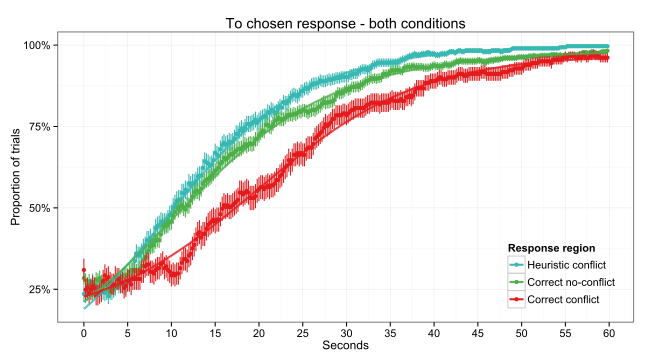
\includegraphics[width=\figurewidth]{imgs/exp6-all-to-chosen.pdf}
  \caption[Proportion of cursor in region of chosen response option, Experiment 6.]{
    \label{fig:exp6-all-to-chosen}
    Proportion of mouse cursors in the region of
    the response option which was ultimately selected on that trial.    
  }
\end{figure}

This time course data also allows us to
supplement the response time analyses reported above
by looking at the speed at which participants moved the mouse cursor to
the region of the response option they eventually did select.
Figure 4 shows this measure for correct responses to no-conflict problems,
and for both heuristic and correct responses to conflict problems.
The curve for each response region over time
was modelled using third-order polynomial logistic regression models
\citep[or growth curves; see][]{Mirman2014},
such that the log odds of the cursor being in that region were given as
$\alpha + \beta_1 t + \beta_2 t^2 + \beta_3 t^3$.
Natural polynomials were used,
meaning that the intercept corresponded to the log odds at 0 seconds,
the linear term to the simple change over time,
and the quadratic and cubic terms to higher-order 'wiggles' later in the time course.%
\footnote{
  One disadvantage of using these natural polynomial terms
  is that they are by definition correlated,
  and so the model suffers from mild multicollinearity,
  which leads to some loss of statistical power.
  However, as the alternative, orthogonal polynomial terms
  would be difficult to interpret individually,
  I believe this approach lends itself
  to a clearer description of the data.
  }

To test for a significant difference between two curves,
a null model, in which the  weights were the same for each curve,
was compared with a full model, in which there were different  weights for each curve.
Chi-squared tests were used to compare the deviance of each model,
with degrees of freedom corresponding to the number of  parameters added in the full model.
Note that $\alpha$, the intercept, was not allowed to vary between curves.
Finally, a random effect for the linear time term was included for each participant,
to allow for individual variability in
how quickly each participant moved towards a response in general.
Random effects on other terms, by participant, or by problem, were considered,
but led to convergence issues, and so only this term,
which was found to account for the most variance, was included.

Mirroring the response time analyses, and as predicted by all dual process accounts,
participant were faster to move towards
the heuristic response option when selecting it
than the correct option for conflict problems
($\chi^2$ = 4515.7, DF = 3, p < .0001),
with the curves differing significantly on the linear, quadratic, and cubic terms
(z's > 5, p's < .0001; see Figure~\ref{fig:exp6-all-to-chosen}).
Again consistent with the response time analyses,
and contrary to previous findings supportive of the intuitive logic model,
participants were faster to move towards the heuristic response on conflict problems
then to move towards the correct response on no-conflict problems
($\chi^2$, DF = 3, p < .0001).
This effect was mainly driven by a significant difference
on the linear term between the curves (z = 2.352, p = .0187).

Most dual process theories, including default-interventionist,
parallel-competitive, and intuitive logic accounts,
would predict that participants should be
drawn towards the heuristic option
on trials where they ultimately give the correct response.
In order to test for this attraction,
I compared the probability over time of
the cursor being in the region of the heuristic option
with the average probability of it being in the region of
either foil option on those trials (Figure~\ref{fig:exp6-correct-not-chosen}).
A higher probability of being in the region of the heuristic option
than the foils constitutes evidence of an attraction towards that heuristic response.
Visual inspection of Figure~\ref{fig:exp6-correct-not-chosen} shows that
this is the case from approximately 10 seconds onwards.
Again, third order polynomial regression models were fit to this data,
which showed that the difference between the curves was statistically significant
($\chi^2$ = 428.2, DF = 3, p < .0001),
with significant differences on the linear, quadratic, and cubic terms
(z's > 2.1, p's < .05).
Therefore, when selecting the correct response,
participants were more drawn to the heuristic option than to the foils,
as predicted both by default-interventionist
and parallel-competitive or intuitive logic accounts.

\begin{figure}[pt]
  \centering
  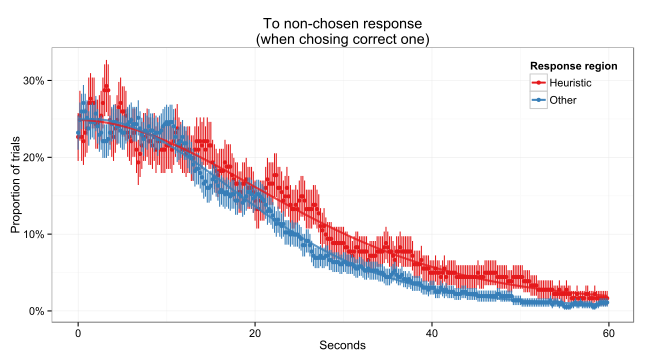
\includegraphics[width=\figurewidth]{imgs/exp6-correct-not-chosen.pdf}
  \caption[Proportion of cursor in region of other response options
  when correct response was given, Experiment 6.]{
    \label{fig:exp6-correct-not-chosen}
    Proportion of trials in the region of each option, over time,
    for trials in which the correct option was eventually chosen,
    for conflict problems.
    Error bars show standard error of measurement.
    Lines show fitted polynomial regression curves.
    Participants were more likely to be in the region of the heuristic response from around 10 seconds onwards.
  }
\end{figure}

\begin{figure}[pb]
  \centering
  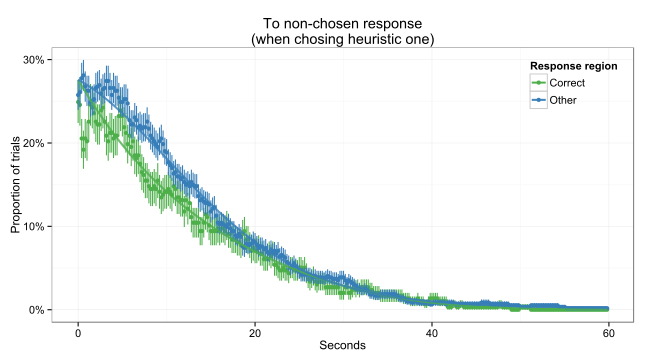
\includegraphics[width=\figurewidth]{imgs/exp6-heuristic-not-chosen.pdf}
  \caption[Proportion of cursor in region of other response options
  when heuristic response was given, Experiment 6.]{
    \label{fig:exp6-heuristic-not-chosen}
    Proportion of trials in the region of each option, over time,
    for trials in which the intuitive option was eventually chosen,
    for conflict problems.
    Participants were less or equally likely to be
    in the region of the correct option than a foil throughout.
  }
\end{figure}


A more interesting comparison is between
the attraction towards the correct response option,
and that towards the foil options,
on conflict trials where the heuristic response is given.
According to the default-interventionist account,
Type 2 processes have not become engaged at this point,
and so the correct response option should not be
any more attractive than the foil options.
According to the parallel-competitive account,
on the other hand, both Type 1 and Type 2 processes
should be engaged on such trials,
and so participants should be drawn towards
giving the response cued by Type 2 processes
(that is, the correct response).
Either result could be consistent with the intuitive logic theory,
depending on the mechanism by which conflict is actually detected.
If conflict detection occurs because
Type 1 processes simultaneously cue both the correct and heuristic responses,
then attraction towards the correct response option should be seen here.
Conversely, if conflict is detected
without Type 1 processes actually producing the correct response,
then the intuitive logic theory,
like the classic default-interventionist account,
would predict no attraction towards the correct response option here.
Of course, no conflict would be predicted by a selective theory.

Figure~\ref{fig:exp6-heuristic-not-chosen} shows that,
contrary to the prediction of the parallel-competitive
and intuitive logic accounts,
participants are not more likely to move towards the correct response option
than either of the foils before giving the heuristic response.
Participants were in fact less likely
to be in the region of the correct option than the foils.
The polynomial regression model showed that
the difference between the curves shown is again significant
($\chi^2$ = 208.0, DF = 3, p < .0001),
with significant differences between the curves on the
linear, quadratic, and cubic terms (z's > 9, p's < .0001).
This result indicates that the correct responses were on average
actually less attractive than the foils.
This is perhaps unsurprising,
given that part of the difficulty of the CRT
lies in the failure of intuition to support the correct response.

%% Finally, once again following previous tests of
%% the intuitive logic theory \citep[e.g.][]{Mevel2014},
%% I repeated the time course analyses reported above for both the
%% ``majority heuristic'' and ``minority heuristic'' participants.
%% The plots for these analyses are shown in Appendix~\ref{appendix:exp6_participants},
%% and reveal that my main findings hold for
%% both sets of participants.
%% \aside{This bit is tricky, especially after the reviews.
%%   Talk about by-item differences here?
%%   Eye balling them, there really is no difference for the bat and ball problems,
%%   but maybe I could test this?}
%% Appendix~\ref{appendix:exp6_items} shows the same analyses
%% plotted separately for each of the eight CRT problems.
%% Again, the results described broadly hold true across all items.
%% However, the bat-and-ball question
%% can be seen to differ slightly from the others
%% in some of the analyses here.
%% I explore this discrepancy in Appendix~\ref{appendix:exp6_items_model}.

\FloatBarrier
